\interlude{Endzeitstimmung}

\begin{frame}[T]{Die Zerstörung der Kryptografie}
% "Warum sind wir eigentlich hier"
% Todo (Karo): Reisserische Youtube Headings Einfügen
%\begin{itemize}
  % \item \url{https://www.youtube.com/watch?v=e-lIgqD5Nxk}
  % \item \url{https://www.youtube.com/watch?v=h6w4SX7ZJMQ}
  % \item \url{https://www.youtube.com/watch?v=-UrdExQW0cs}
  % \item \url{https://www.youtube.com/watch?v=05Uy-hFFkRU}
  % \item \url{https://www.youtube.com/watch?v=ON5pVc9bIRo}
    % - "Lehrer: Subjekt, prädikat, objekt – Der Satz ist unvollständig"
  % - Hier geht es viel um Bitcoiin.
    % - Wir kryptografen sind ja nicht so glücklich darüber, dass die Bitcoin-Bros uns das Kürzel gestohlen haben
% \end{itemize}
\only<1>{
	  \ImgSource{%
			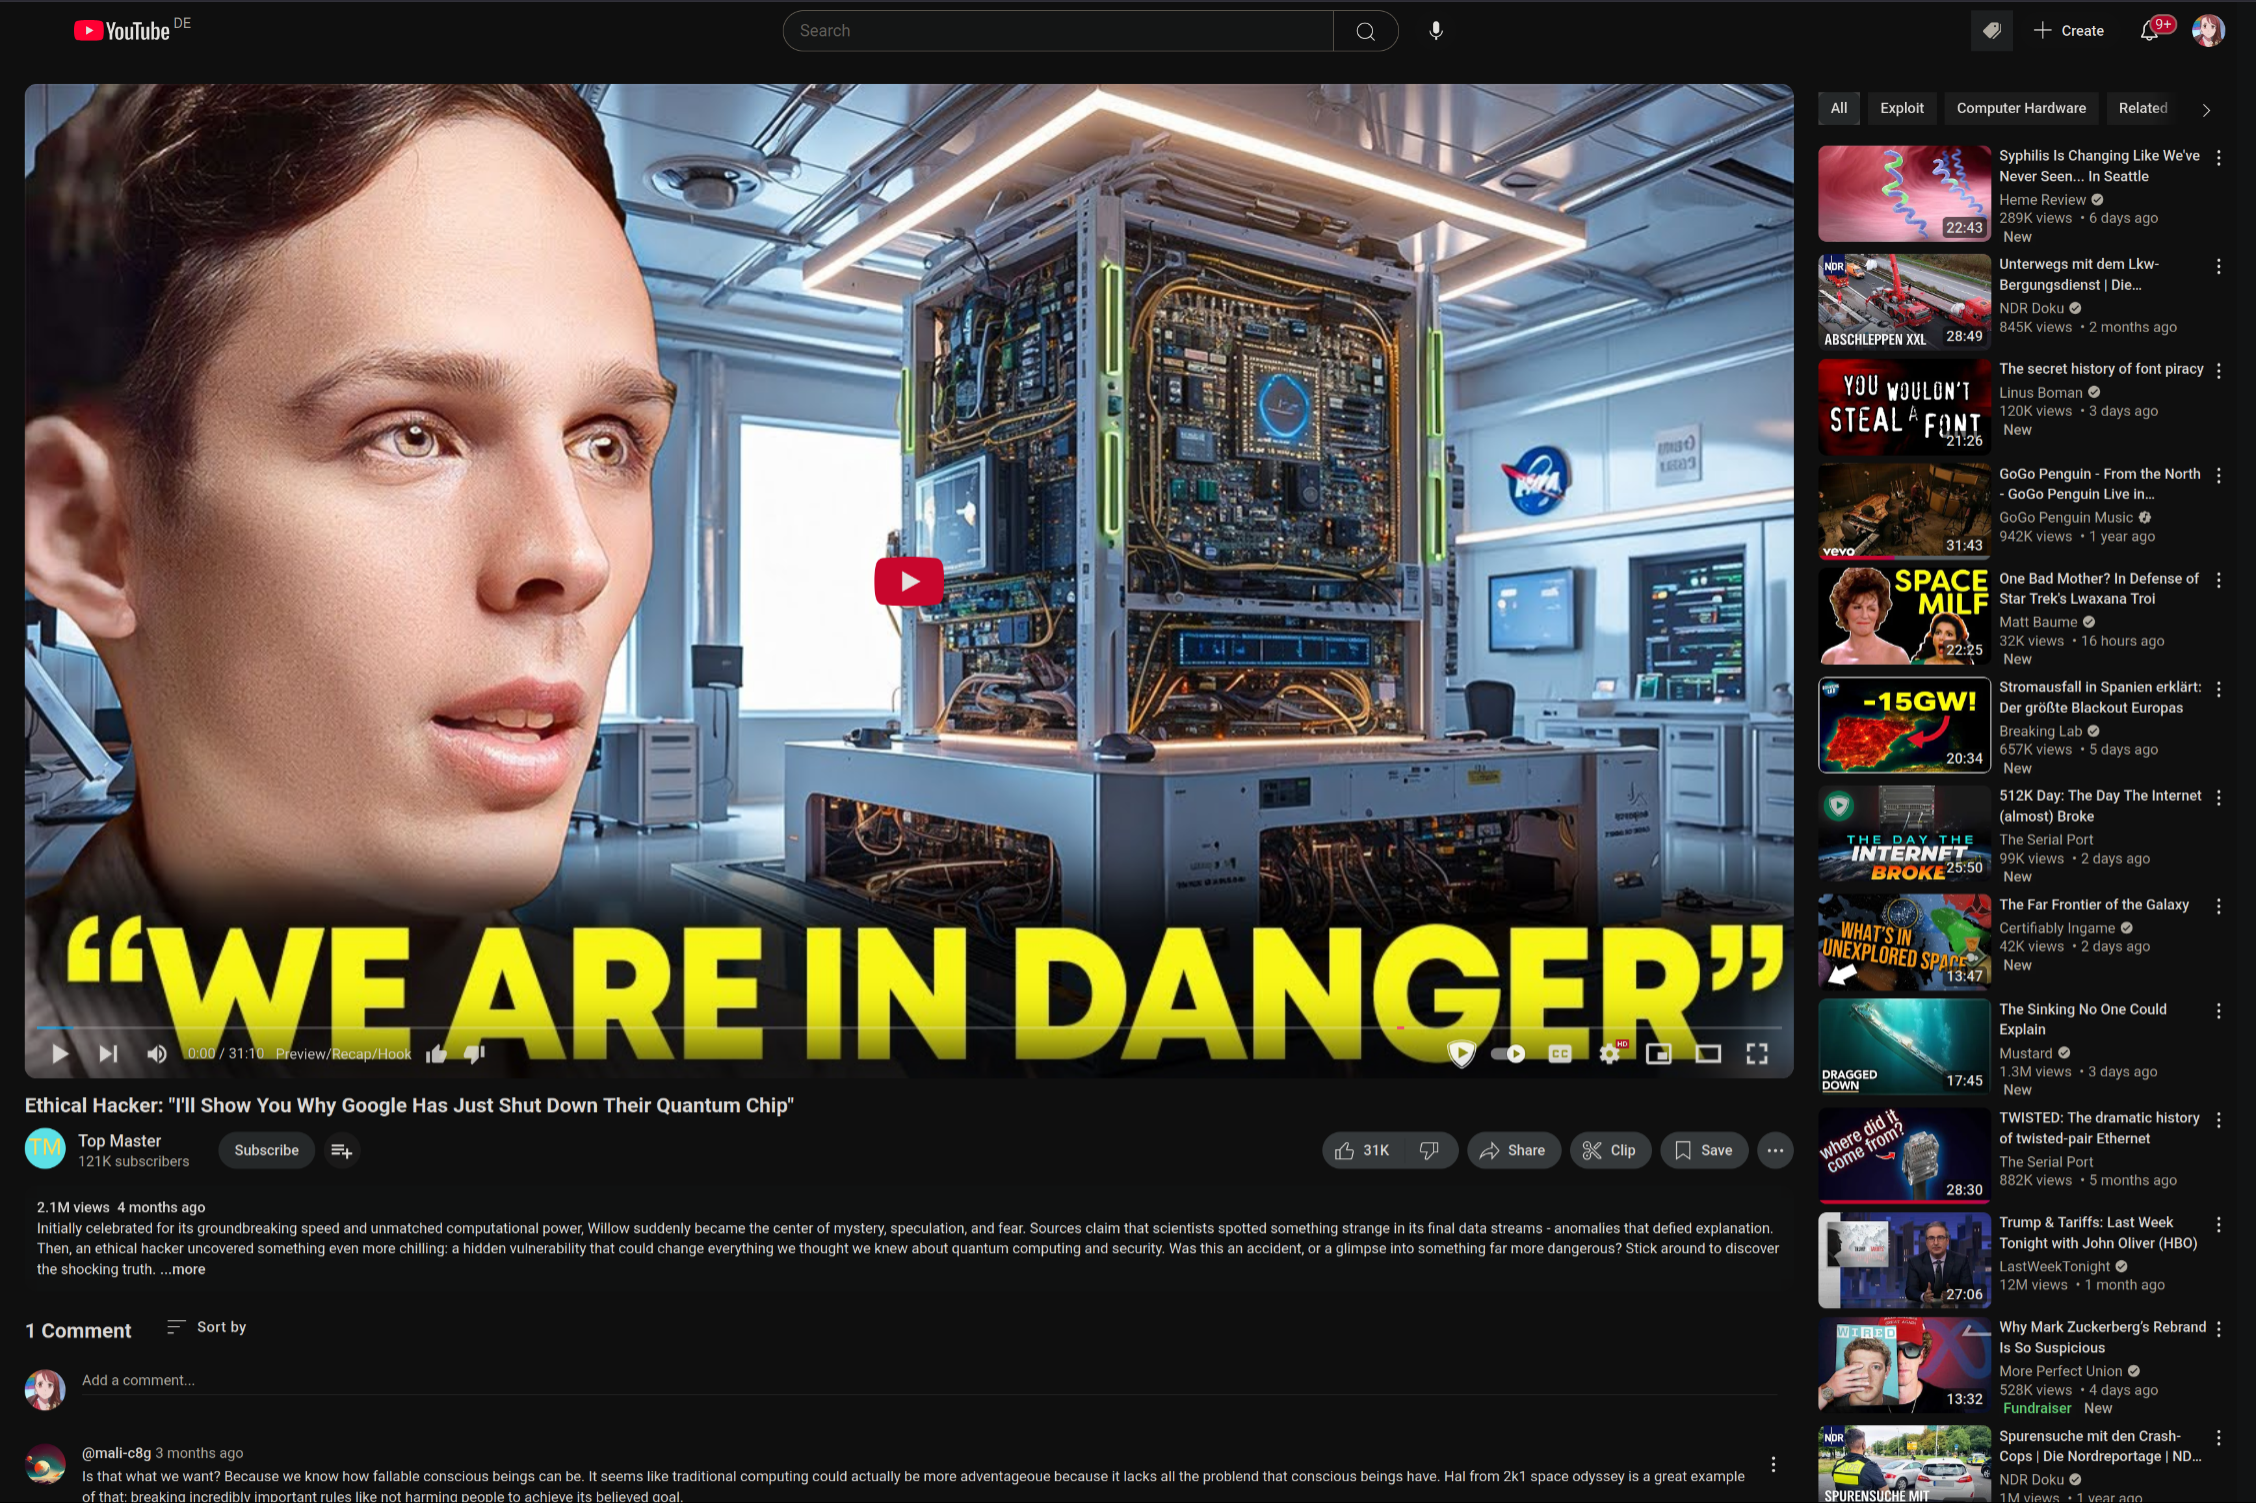
\includegraphics[height=\defaultframetextheight,trim=10 350 400 62,clip]{graphics/quantastropy-yt-screenshots/we-are-in-danger.png}}{https://www.youtube.com/watch?v=h6w4SX7ZJMQ}}
\only<2>{%
 	\ImgSource{%
	  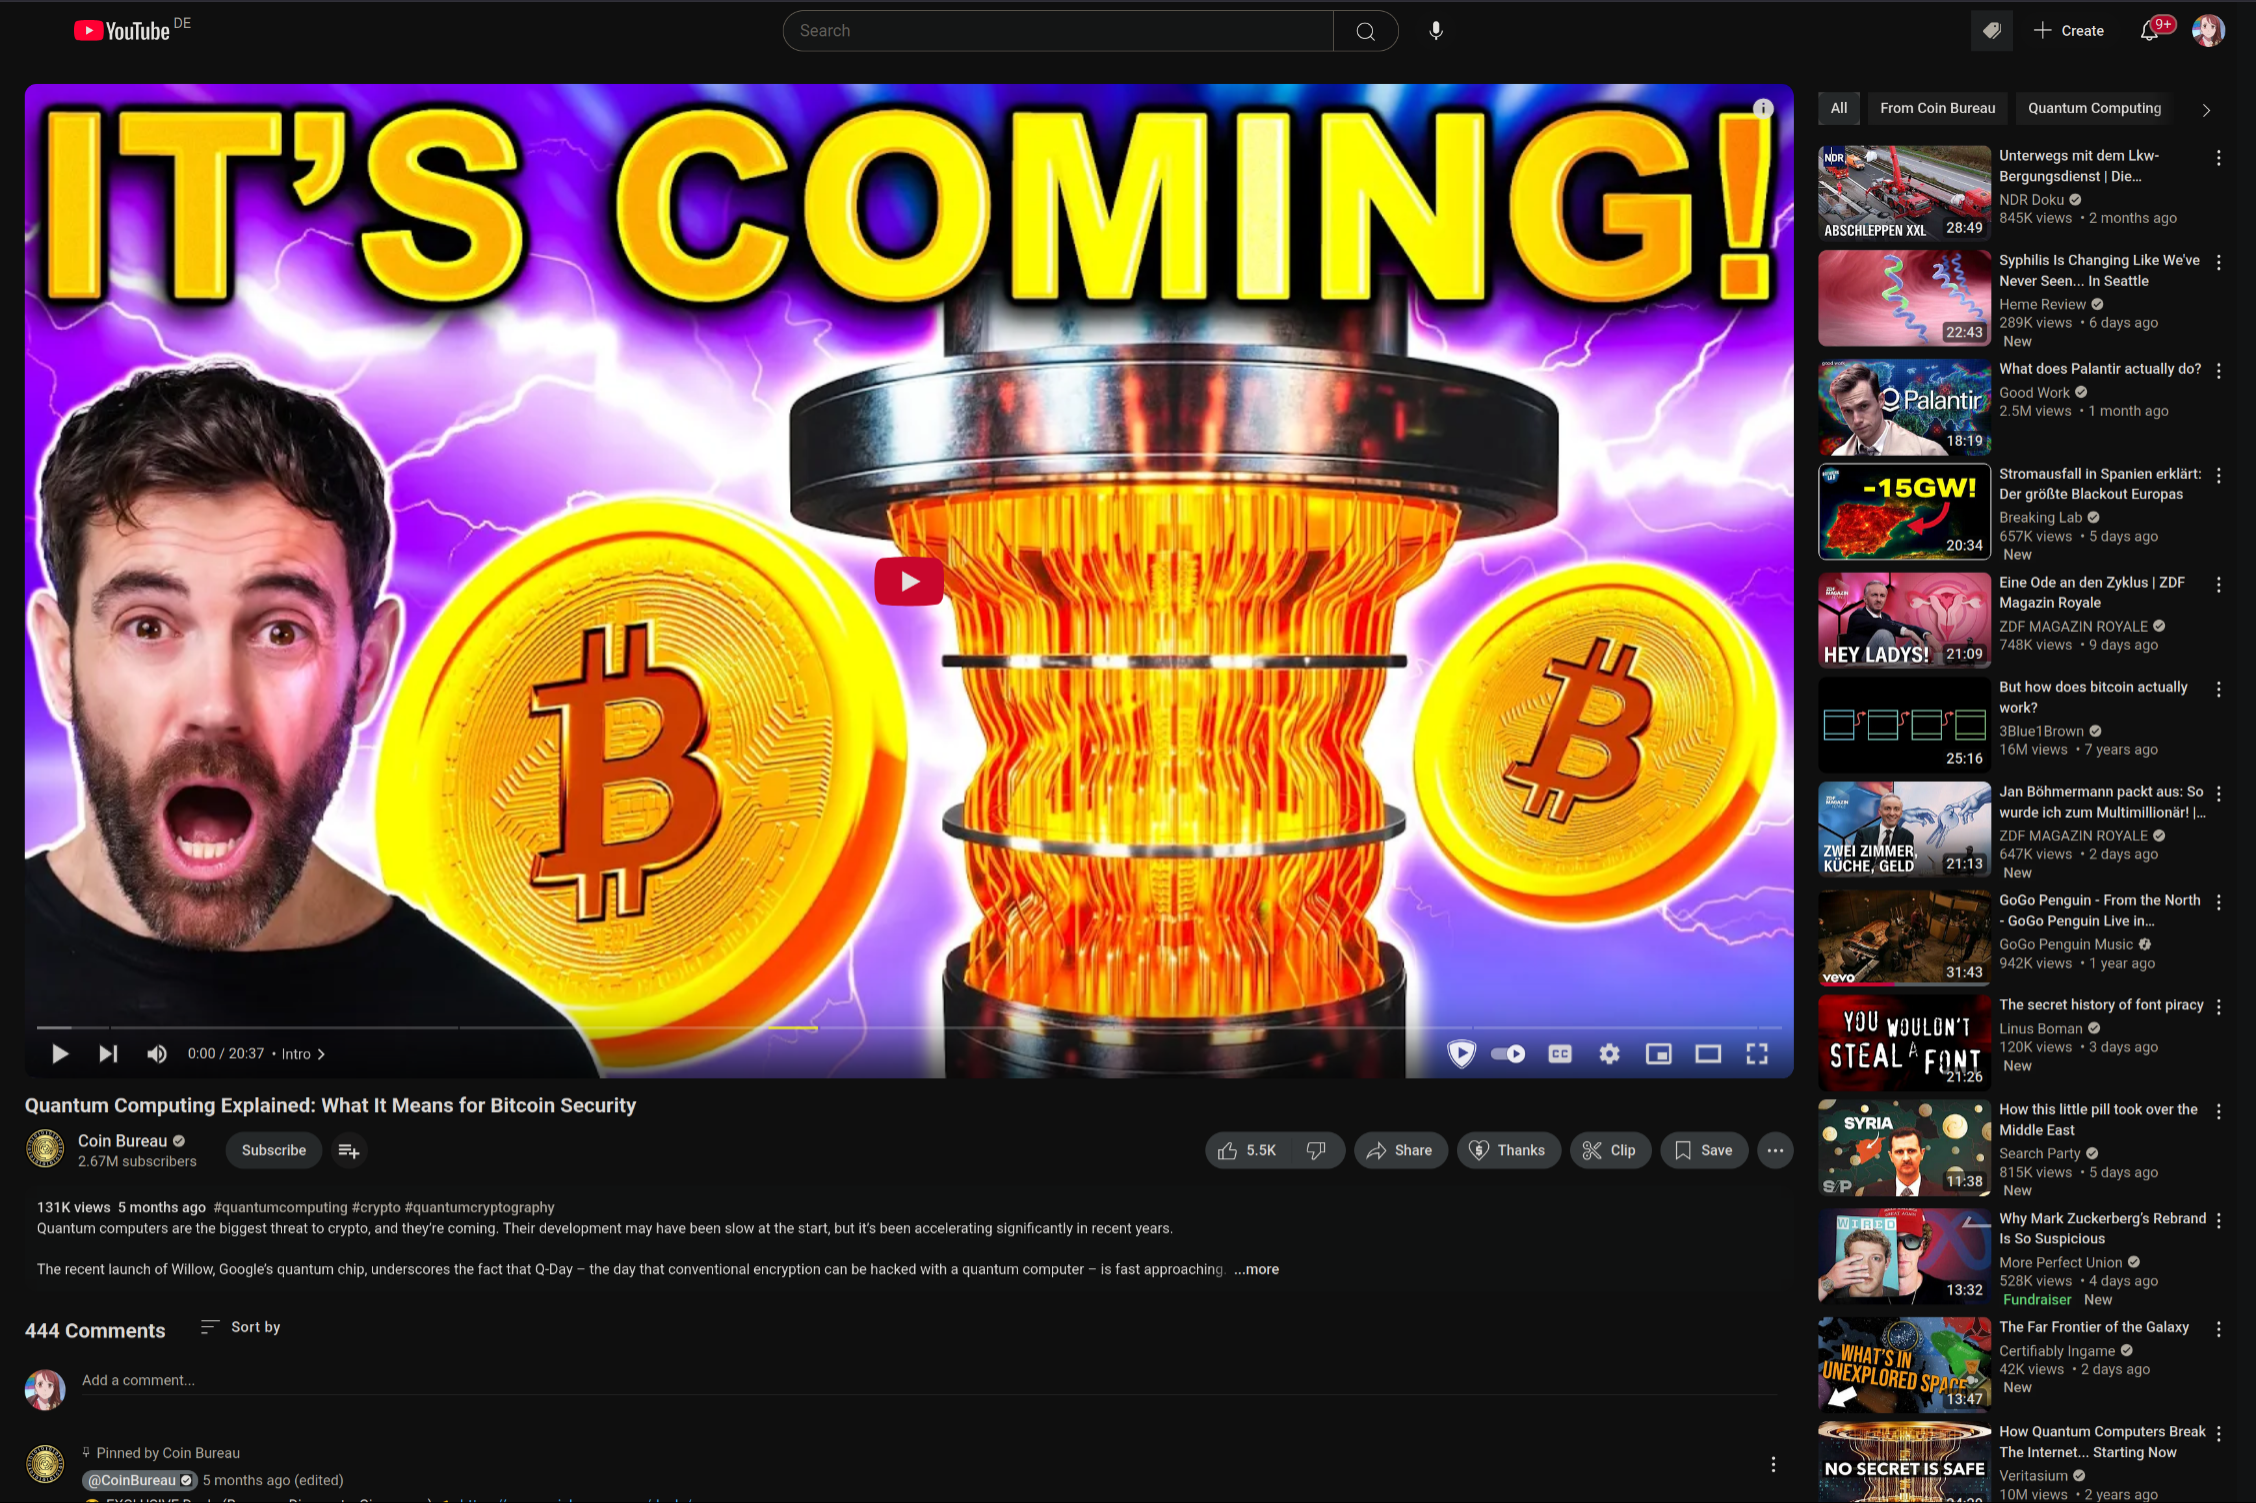
\includegraphics[height=\defaultframetextheight,trim=10 350 400 62,clip]{graphics/quantastropy-yt-screenshots/it-is-coming.png}}{https://www.youtube.com/watch?v=ON5pVc9bIRo}}
\only<3>{%
 	\ImgSource{%
  	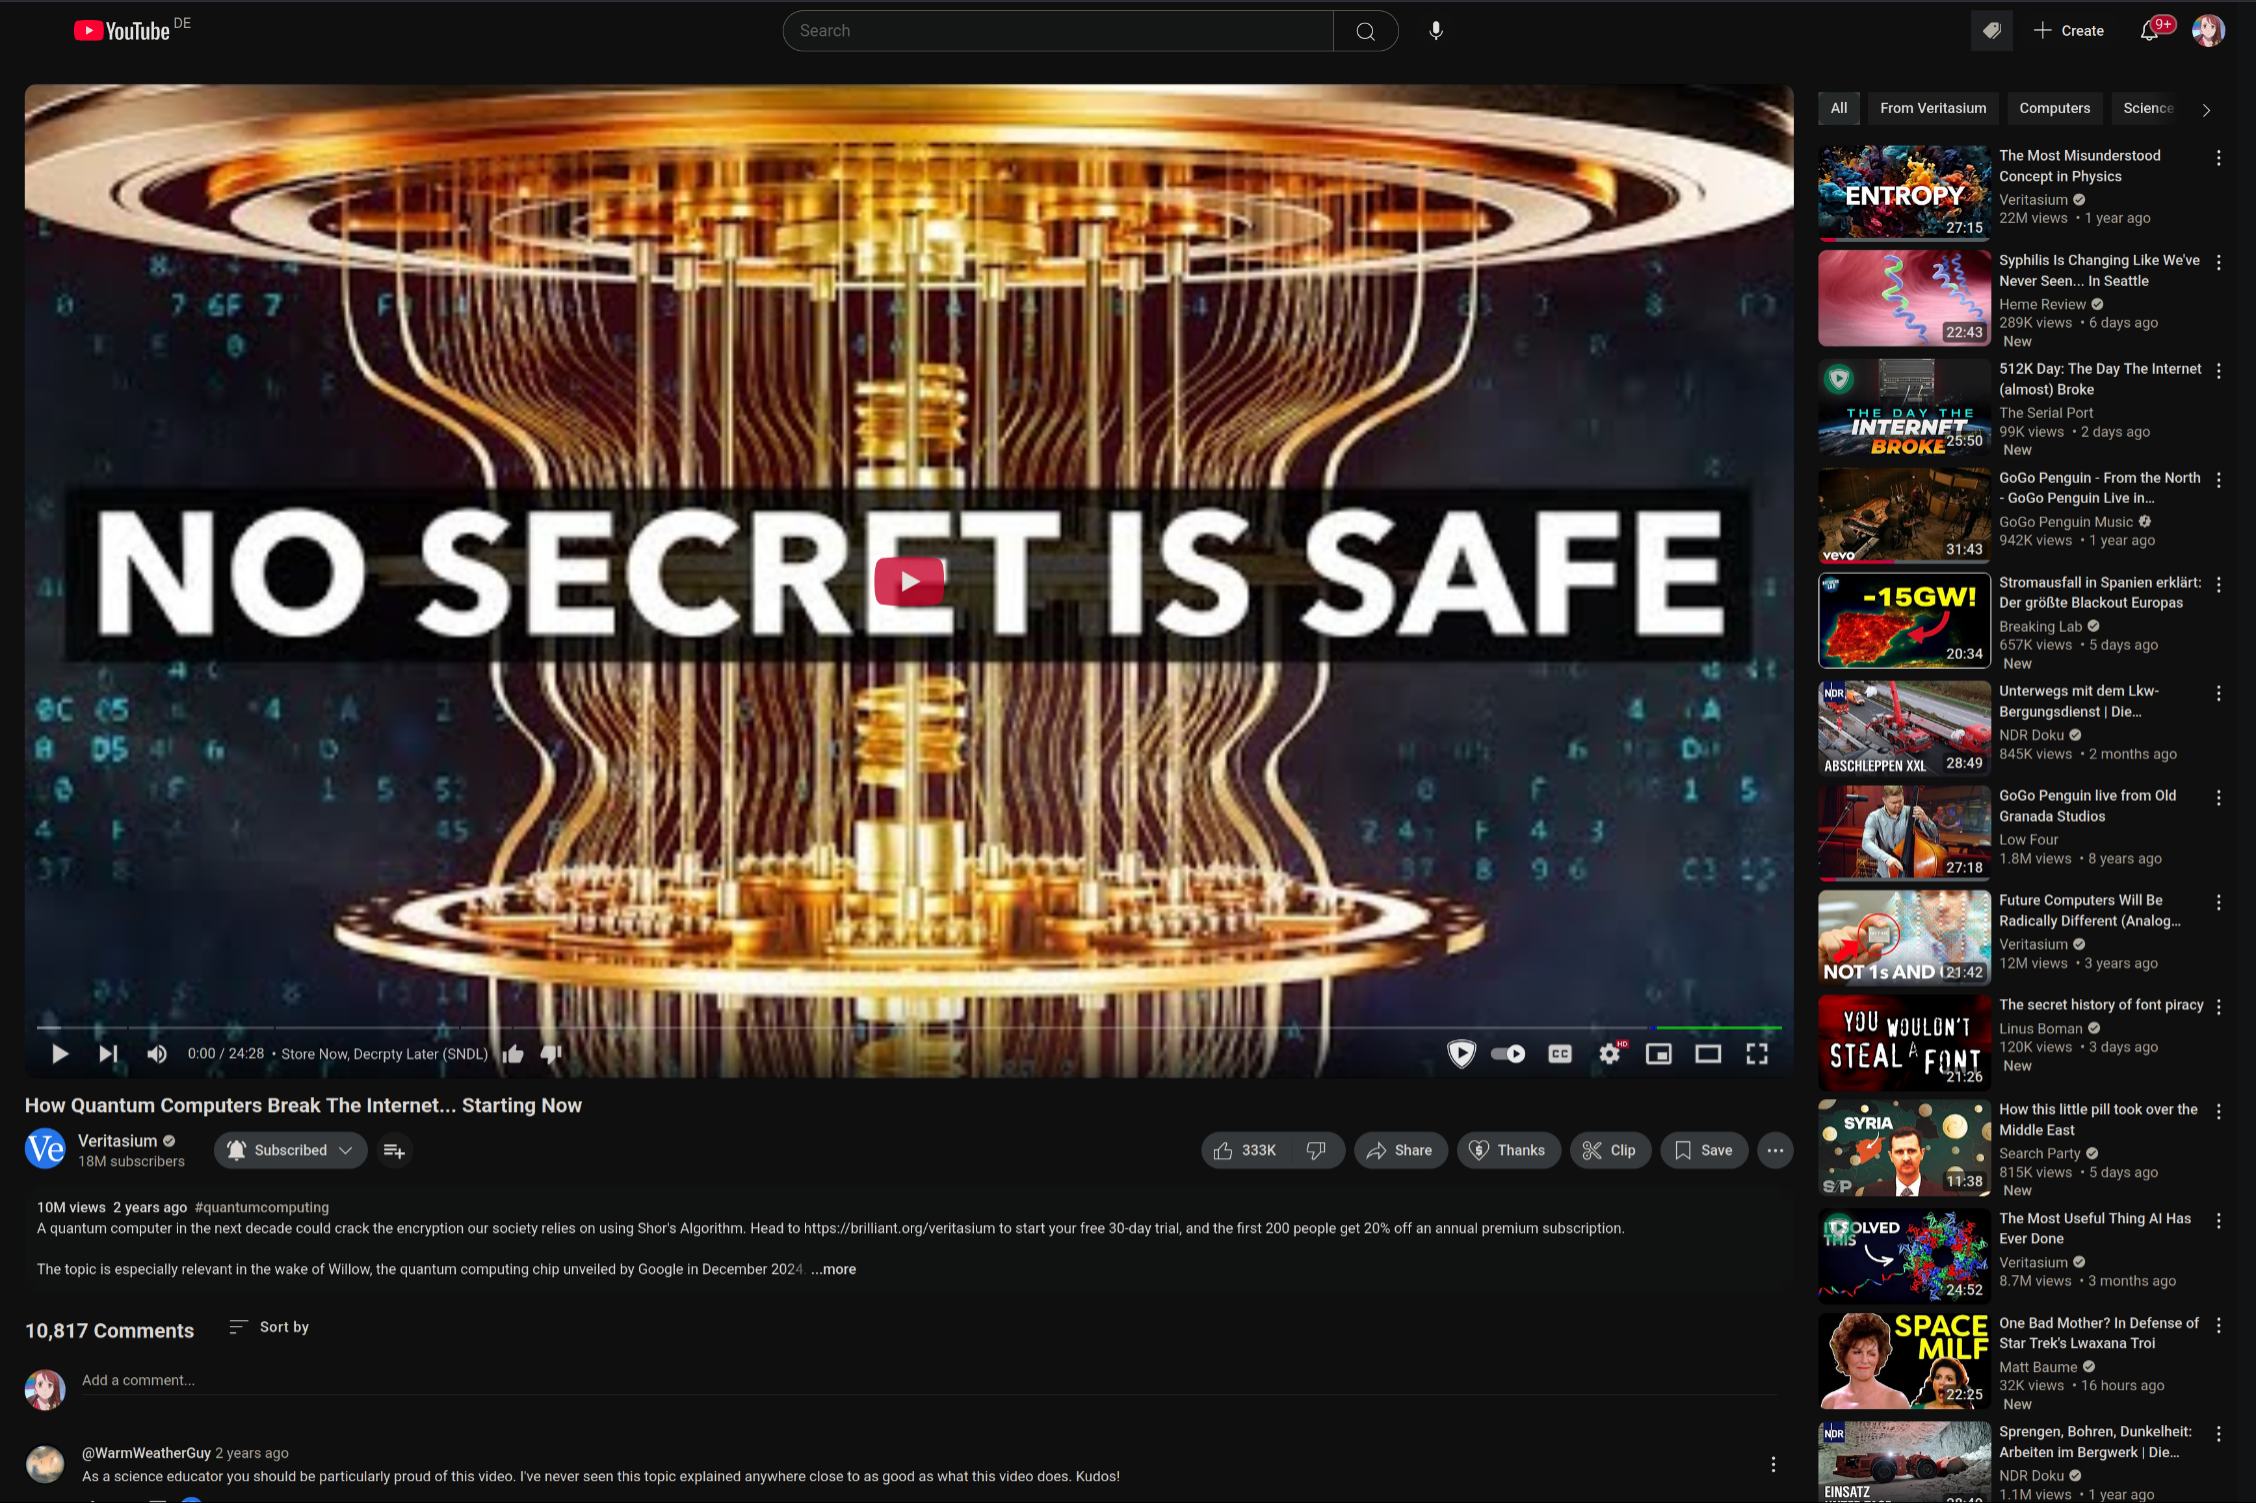
\includegraphics[height=\defaultframetextheight,trim=10 350 400 62,clip]{graphics/quantastropy-yt-screenshots/no-secret-is-safe.png}}{https://www.youtube.com/watch?v=-UrdExQW0cs}}
\end{frame}

% \begin{frame}[T]{Quantencomputer – Shors Algorithmus}

% \begin{itemize}
%   \item Kann speziefische Kryptografische Primitiven Angreifen
%   \item Schneller als Exponenziell
%   \item Erfunden 1994
%   \item Gegenmaßnahme existieren seit 1978 (das wussten wir damals nur nicht)
%   \item Es ist teuer und komplex die in den Einsatz zu bringen
%   \item => Diese komponenten werden Flächendeckend eingesetzt
% \end{itemize}

% Bild: 
% \begin{itemize}
%   \item Physiker: Mein Gerät lässt Flugzeuge mit RS 25 McGuffin Triebwerken abstürzen
%   \item Manager: RS 26 McGuffin Triebwerke sind so viel teurer. Niemand wird migrieren wollen.
%   \item Physiker: Halt dich ran, ich brauche nur 40 Jahre um das zu bauen!
% \end{itemize}

% \end{frame}

\begin{frame}[T]{Quantencomputer – So schnell wie Fusion}
  
  \ImgSource{%
		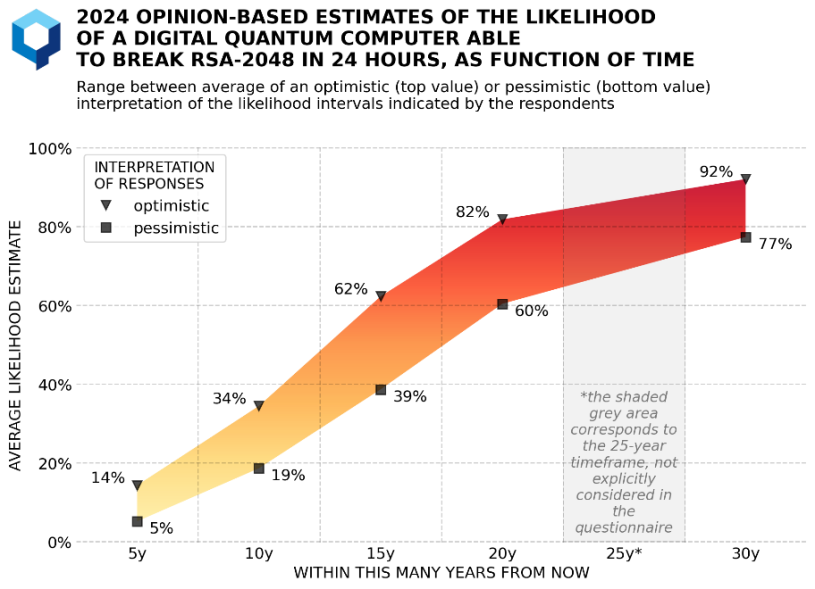
\includegraphics[height=\defaultframetextheight,clip,trim=0  0 0 120]{graphics/quantum-timeline.png}
	}{https://globalriskinstitute.org/publication/2024-quantum-threat-timeline-report/}
% \ImgSource{\includegraphics[height=.8\textheight]{assets/xkcd_678.png}}{https://xkcd.com/678/}
%
%\ImgSource{https://globalriskinstitute.org/publication/2024-quantum-threat-timeline-report/}}
%Quelle: \url{https://globalriskinstitute.org/publication/2024-quantum-threat-timeline-report/}

\end{frame}


\begin{frame}[T]{Unsere vernetzte Welt steht still}
  \begin{columns}[T,fullwidth]
    \begin{column}{.55\linewidth}
      \includegraphics[height=1.05\defaultframetextheight,trim=43 20 0 0]{comic/rosenpass-comic-earth-stop.png}
    \end{column}
    \begin{column}{.45\linewidth}
      \vspace{10em}
      \begin{itemize}
        \setlength{\itemindent}{-1.2ex}
        \item Wir arbeiten im Internet
        \setlength{\itemindent}{-2ex}
        \item Steuern damit kritische Infrastruktur
        \setlength{\itemindent}{-3.8ex}
        \item Unsere Lieferketten verlassen sich darauf
      \end{itemize}
    \end{column}
    \hfill
  \end{columns}
\end{frame}


\begin{frame}[T]{Angreifer, die Hamstern}

  \begin{columns}[T,fullwidth]
    \hfill
    \begin{column}{.5\textwidth}
      \vspace{4em}
      \begin{itemize}
        \item Angreifer können verschlüsselte Daten auf Vorrat speichern
        \vspace{.8em}
        \item So werden Angriffe auf vergangene Kommunikation möglich
        \vspace{.8em}
        \item \say{Store now, decrypt later Attack}
      \end{itemize}
    \end{column}

    \begin{column}{.6\textwidth}
      \vspace{4em}
      \reflectbox{
        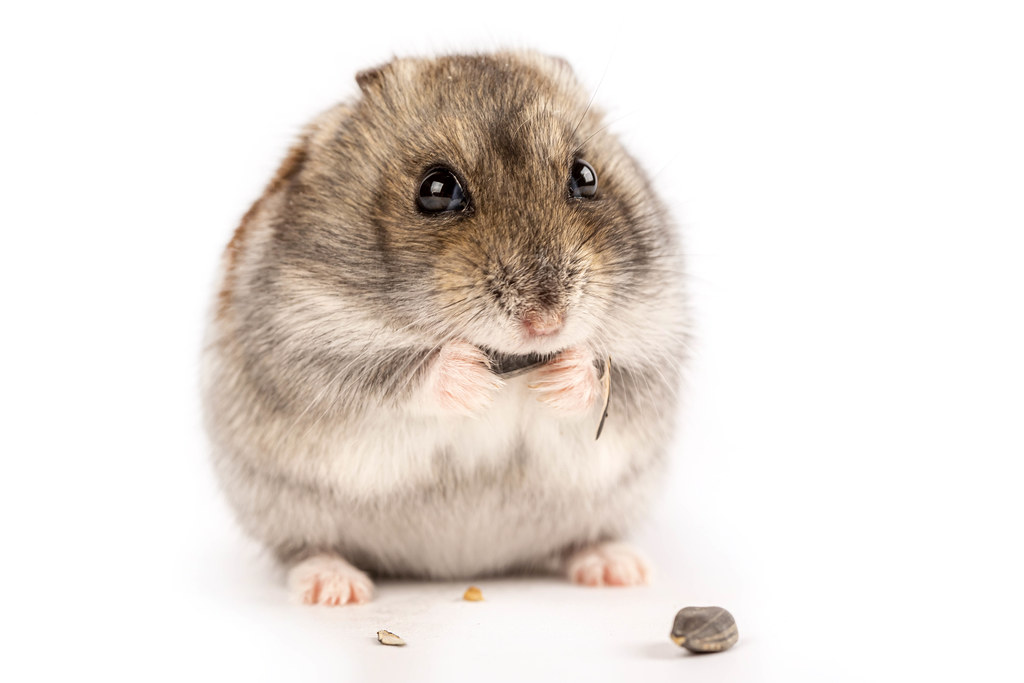
\includegraphics[height=.8\textheight,trim=0 130 300 0,clip]{graphics/gray-hamster-eating-sunflower-seed.jpeg}
      }
    \end{column}
  \end{columns}

\end{frame}
